\documentclass[12pt]{article} \usepackage[utf8]{inputenc}
\usepackage{fullpage}
\usepackage{parskip}
\usepackage{amsmath,amssymb,mathtools}
\usepackage{microtype}
\usepackage{booktabs}
\usepackage{graphicx,subcaption}
\usepackage{algorithm}
\usepackage[round]{natbib}
\usepackage{tikz-cd}


\usepackage[most]{tcolorbox}
\newtcolorbox[]{solution}[1][]{%
    breakable,
    enhanced,
    colback=white,
    title=Solution,
    #1
}
\usepackage{xcolor} %hilight
\newcommand{\hilight}[1]{\colorbox{yellow}{#1}}
%% ---------------------------------
%\begin{solution}
%\hilight{TODO}
%\end{solution}
%% ---------------------------------



\usepackage{tikz}
\usetikzlibrary{bayesnet}

\newcommand*\circled[1]{
\tikz[baseline=(char.base)]{\node[shape=circle,draw,inner sep=1pt] (char) {#1};}
}
            
 
% xun
\newcommand{\Gcal}{\mathcal{G}}
\newcommand{\Ical}{\mathcal{I}}
\newcommand{\Hcal}{\mathcal{H}}
\newcommand{\Ucal}{\mathcal{U}}
\newcommand{\Tcal}{\mathcal{T}}
\newcommand{\Ncal}{\mathcal{N}}
\newcommand{\Xcal}{\mathcal{X}}
\newcommand{\Cbs}{\boldsymbol{C}}
\newcommand{\Sbs}{\boldsymbol{S}}
\newcommand{\Pa}{\text{Pa}}
\newcommand{\De}{\text{De}}
\newcommand{\Nd}{\text{Nd}}
            

\title{10-708 PGM (Spring 2019): Homework 1
{\color{red} v1.1}
}
\author{
\begin{tabular}{rl}
Andrew ID: & Moroccan Student\\
Name: & [Belcaid Anass] \\
Collaborators: & [Working alone]
\end{tabular}
}
\date{}


\begin{document}

\maketitle



\section{Bayesian Networks [20 points] (Xun)}

State True or False, and briefly justify your answer in a few sentences. You can cite theorems from \citet{koller2009probabilistic}. Throughout the section, $P$ is a distribution and $\Gcal$ is a BN structure. 

\begin{enumerate}

\item \textbf{[2 points]} If $ A \perp B \ | \ C $ and $ A \perp C \ | \ B $, then $ A \perp B $ and $ A \perp C $. 
(Suppose the joint distribution of $ A, B, C $ is positive.)

\begin{solution}
 \textbf{True}, as this a special case for the \textbf{contraction} theorem
 on~\cite{koller2009probabilistic}. 
\[
  (X \perp Y | Z, W)\;\&\;(X \perp Z | Y, W) \Longrightarrow (X \perp Y, Z | W)
\]

We simply take $X=A$, $B=Y$, $C=Z$ and $W$ is a sure event. We then get

\[
  (A \perp B, C)
\]

\end{solution}

\begin{figure}[h]
\centering
\begin{tikzcd}
A \arrow[r] & B \arrow[r] & C \\
D \arrow[ur] \arrow[r] & E & 
\end{tikzcd}
\caption{A Bayesian network.}
\label{fig:y-bayesnet}
\end{figure}


\item \textbf{[2 points]} In Figure~\ref{fig:y-bayesnet}, $ E \perp C \ | \ B $.

\begin{solution}
  \textbf{True}, As any path to $C$ is blocked by $B$ the unique parent to
  $C$.
\end{solution}

\item \textbf{[2 points]} In Figure~\ref{fig:y-bayesnet}, $ A \perp E \ | \ C $.

\begin{solution}
 \textbf{False}, There is an active trail using the $V$-structure
 $A\rightarrow B \leftarrow D$.
 This structure is activated a child of $B$, which is $C$, is activated.
 Hence the trail $A-B-D-E$ is active.
\end{solution}



\begin{figure}[h]
\centering
\begin{tikzcd}
P \text{ factorizes over } \Gcal  
\arrow[r, Rightarrow, "(1)"] 
& \Ical (\Gcal) \subseteq \Ical (P) 
\arrow[r, Rightarrow, "(2)"] 
& \Ical_\ell (\Gcal) \subseteq \Ical (P)
\arrow[ll, Rightarrow, bend left=30, "(3)" above]
\end{tikzcd}
\caption{Some relations in Bayesian networks.}
\label{fig:relations-bayesnet}
\end{figure}



\item \textbf{[2 points]} In Figure~\ref{fig:relations-bayesnet}, relation (1) is true.

\begin{solution}
  \textbf{True}, direct result of  the theorem (3.2) on~\cite{koller2009probabilistic}.
\end{solution}
\item \textbf{[2 points]} In Figure~\ref{fig:relations-bayesnet}, relation (2) is true.

\begin{solution}
  \textbf{True}, If the set of independences by the d-separation are
  verified in a distribution $P$, then $P$ must also verify the local
  independences in the Bayesian graph.
\end{solution}
\item \textbf{[2 points]} In Figure~\ref{fig:relations-bayesnet}, relation (3) is true.

\begin{solution}
  \textbf{True}. Direct result of theorem (3.1)
  on~\cite{koller2009probabilistic}
\end{solution}

\item \textbf{[2 points]} If $ \Gcal $ is an I-map for $ P $, then $ P $ may have extra conditional independencies than $ \Gcal $.


\begin{solution}
  \textbf{True}, As the definition of I-map only forces $P$ to verify all the
  of independences in $\Gcal$. $P$ could have additional hidden
  independences that are not reflected in the graph.
\end{solution}

\item \textbf{[2 points]} Two BN structures $ \Gcal_1 $ and $ \Gcal_2 $ are I-equivalent iff they have the same skeleton and the same set of v-structures.

\begin{solution}
  \textbf{False}, the $v$-structure is not sufficient here, as in one graph
  the parents could be connected and not in the other one. The correct
  theorem (3.8)~\cite{koller2009probabilistic} states that two graphs are
  $I$-equivalent if they have the same skeleton and the same
  \textbf{immoralities}.
\end{solution}

\item \textbf{[2 points]} The minimal I-map of a distribution is the I-map with fewest edges.

\begin{solution}
  \textbf{False}, a minimal map simply means that it can accept an edge
  removal to be an $I$-map. Since this map is not unique, we could find
  several $I$-maps with different number of edges. 
\end{solution}
\item \textbf{[2 points]} The P-map of a distribution, if exists, is unique. 
\begin{solution}
  \textbf{False}. From~\cite[page 84]{koller2009probabilistic}, the $P$-map
  is unique up to $I$-equivalence between networks.
\end{solution}
\end{enumerate}


\newpage


\section{Undirected Graphical Models [25 points] (Paul)}

\subsection{Local, Pairwise and Global Markov Properties [18 points]}

\begin{enumerate}
    \item Prove the following properties:
    \begin{itemize}
        \item \textbf{[2 points]} If $A \perp {\color{red} (B,D) } \ | \ C$ then $A \perp B \ | \ C$.
        \begin{solution}
          \small
         \begin{eqnarray*}
           P(A, B|C) &=& \sum_d P(A, B|C,D) P(D) \\
                     &=& \sum_d P(A|B,C,D) P(B|C,D) P(D)\\
                     &=& \sum_d P(A|C) P(B|C,D)P(D)\\
                     &=& P(A|C) \sum_d P(B|C,D)P(D)\\
                     &=& P(A|C) P(B|C)
         \end{eqnarray*} 
        \end{solution}
        \item \textbf{[2 points]} If $A \perp {\color{red} (B,D) } \ | \ C$ then $A \perp B \ | \ {\color{red} (C,D) }$ and $A \perp D \ | \ {\color{red} (B,C) }$.
      \begin{solution}
        We have
        \begin{eqnarray}
          P(A,B,D|C) &=&  P(A,B|D,C)P(D)\\
                     &=& P(A|C,D) P(B|C,D) P(D)
        \end{eqnarray}
        From the equatlity  between line (1) and (2), we could conclude
        that 
      \[
      P(A,B|C,D) = P(A|C,D) P(B|C,D)
      \]
      the same proof, is applied for $D$.
      \end{solution}
        \item \textbf{[2 points]} For strictly positive distributions, if $A \perp B \ | \ {\color{red} (C,D) }$ and $A \perp C \ | \ {\color{red} (B,D) }$ then $A \perp {\color{red} (B,C) } \ | \ D$.
          \begin{solution}
          using the chain rule we can write:
            \begin{eqnarray*}
              P(A,B,C|D) &=& P(A|B,C,D) P(B,C|D)\\
                         &=& P(A|D) P (B,C|D,A)
            \end{eqnarray*}
            In the secon equation since $A \perp B | (C,D)$ and $A \perp C|
            (B,D)$, we could conclude that $P(B,C|D,A) = P(B,C|D)$. Now we
            combine both equations we found that 
            \[
              P(A|B,C,D)P(B,C|D) = P(A|D)P(B,C|D)
            \]
            Hence, we conclude that $A\perp (B,C) | D$
          \end{solution}
    \end{itemize}
    \item \textbf{[6 points]} Show that for any undirected graph $G$ and distribution $P$, if $P$ factorizes according to $G$, then $P$ will also satisfy the global Markov properties of $G$.

      \begin{solution}
        Let $(X,Y,Z)$ three disjoint sets in $\Xcal$ such as $Z$
        separates $X$ and $H$ in the markov model $\Hcal$. We shoud
        proove that $P \models (X \perp Y|Z)$

      \begin{enumerate}
        \item As a first case, we consider $X\cup Y \cup Z=\Xcal$, As
          $Z$ separates $X$ and $Y$,  any clique is either in $X\cup Z$ or
          $Y\cup Z$. We denote $\Ical_X$ the set of indices in
          $X\cup Z$ and do the same $\Ical_Y$ for $Y$. Then we could
          write the ditribution $P$ such as:
          \[
            P(X_1,\ldots,X_n) = \frac{1}{Z}
            \prod_{i\in\Ical_X}\phi(D_i)\prod_{i\in\Ical_Y}\phi(D_i)=
            \frac{1}{Z}f(X,Z)f(Y,Z)
          \]
          Which proves that $X$ and $Y$ are independant given $Z$.
        \item If $X\cup Y \cup Z \subset \Xcal$, then we denote the
          set $U = X - (X \cup Y \cup Z)$. We could divice the $U=U_1
          \cup U_2$ such as $U_1$ is connected to $X$ and $U_2$ is
          connected to $Y$. By doing so, we present the same
          argument where $U_1$ will be added to $\Ical_X$ and $U_2$
          to $\Ical_Y$.
      \end{enumerate}
      \end{solution}
    \item \textbf{[6 points]} Show that for any undirected graph $G$ and distribution $P$, if $P$ satisfies the local Markov property with respect to $G$, then $P$ will also satisfy the pairwise Markov property of $G$.

      \begin{solution}
       Let $X$ and $Y$ to be two nodes from the Markov network
       $\Hcal$. 

       \begin{itemize}
         \item If $X$ is connected to $Y$ then by the local markov
           property we have
           \[
             \big(X \perp Y| MB_{\Hcal}(X)) \Longrightarrow (X \perp Y
             | \Xcal - (X,Y)\big)
           \]
          \item If $X$ and $Y$ are not connected. They are necesseraly
            separated by the rest of the nodes in $\Xcal$.
            \[
              \big(X\perp Y | \Xcal - (X,Y)\big)
            \]
       \end{itemize}
      \end{solution}
\end{enumerate}

\subsection{Gaussian Graphical Models [7 points]}

Now we consider a specific instance of undirected graphical models. Let $X = \{ X_1, ..., X_d \}$ be a set of random variables and follow a joint Gaussian distribution $X \sim \mathcal{N}(\mu, \Lambda^{-1})$ where $\Lambda \in \mathbb{S}^{++}$ is the precision matrix. Let $X_j,X_k$ be two nodes in $X$, and $Z = \{X_i \ | \ i \notin \{j,k\}\}$ denote the remaining nodes. Show that $X_j \perp X_k \ | \ Z$ if and only if $\Lambda_{jk} = 0$.

\begin{solution}
  \begin{itemize}
    \item $(X_j \perp X_k\;|\;Z) \Longrightarrow
      \Lambda_{jk}=0$
      Conditioning on $Z$ will reduce the joint probability on
      $(X_j, X_k)$ to a Gaussian with the same precision $\Lambda$ which
      is reduced to the set $(j,k)$ and coefficient are scaled by a
      factor to ensure normalization.
      \[
        \Lambda_{ij}= \text{Cst} \begin{pmatrix} \lambda_{ii} &
          \lambda_{ij}\\
          \lambda_{ij} & \lambda_{jj}\\
        \end{pmatrix}
      \]
    The probability $(X_j, X_k|Z)$ is given by 
    \[
      P(X_j,X_k|Z) = \text{Cst}\exp\big(\Lambda_{jj}(x_j - \mu_j)^2 + 
      \Lambda_{kk} (x_k - \mu_k)^2
      + 2\Lambda_{jk}(x_k-\mu_k)^T(x_j-\mu_j)
    \big)
    \]
    But we know that $(X_j\perp X_k|Z)$, hence the third term must be
    null. Which implies that $\Lambda_{jk}= 0.$
  \item  The inverse $\Lambda_{jk}=0\Longrightarrow (X_j \perp X_k | Z)$
    follows directly from this property as

    \begin{eqnarray}
      P(X_j, X_k|Z) &=& \text{Cst}\exp (\Lambda_{jj}(x_j-\mu_j)^2 +
    \Lambda(x_k -\mu_k)^2) \\
                    &=&
                    \text{Cst}\exp(\Lambda_{jj}(x_j-\mu_j)^2)
                    \exp( \Lambda(x_k -\mu_k)^2)\\
                    &=& P(X_j|Z)P(X_k|Z)
  \end{eqnarray}
  \end{itemize}
\end{solution}


\newpage

\section{Exact Inference [40 points] (Xun)}

\subsection{Variable elimination on a grid [10 points]}

Consider the following Markov network:

\begin{figure}[h]
\centering
\begin{tikzcd}
A \arrow[r, dash] & B \arrow[r, dash] & C \\
D \arrow[r, dash] \arrow[u, dash] & E \arrow[r, dash] \arrow[u, dash] & F \arrow[u, dash] \\
G \arrow[r, dash] \arrow[u, dash] & H \arrow[r, dash] \arrow[u, dash] & I \arrow[u, dash]
\end{tikzcd}
\end{figure}


We are going to see how \emph{tree-width}, a property of the graph, is related to the intrinsic complexity of variable elimination of a distribution. 


\begin{enumerate}

\item \textbf{[2 points]} Write down largest clique(s) for the elimination order $ E, D, H, F, B, A, G, I, C $.

\begin{solution}
    The larget clique for the this elimination will be $(A, B, C, G, I)$
    after eliminating the node $\mathbf{H}$.
  
\end{solution}

\item \textbf{[2 points]} Write down largest clique(s) for the elimination order $ A, G, I, C, D, H, F, B, E $. 

\begin{solution}
  This ordering is amazing keeping the maximum clique at most order
  $\mathbf{3}$. From the first elimination $A$ we get the a maximal clique
  $BDE$. After each node will remove a simple node and keep cliques at most
  of lenght $3$.
\end{solution}

\item \textbf{[2 points]} Which of the above ordering is preferable? Explain briefly. 

\begin{solution}
  The \textbf{second} oredering is clearly better as the complexity of the
  elimination algorithm is determined by $n^K_{\text{max}}$ where
  $n$ is the cardinality of the random variables and $K_{\text{max}}$ is the
  size of the maximal clique.
\end{solution}

\item \textbf{[4 points]} Using this intuition, give a reasonable $ (\ll n^2) $ upper bound on the tree-width of the $ n \times n $ grid. 

  \begin{solution}
   Since we process the cliques from the extremities, we assure that the
   nodes from the left, if we divide the square by half, will never be
   connected to the right part. Hence the maximal tree width will be at
   most $\mathbf{\dfrac{n}{2}}$ 
  \end{solution}


\end{enumerate}

\subsection{Junction tree in action: part 1 [10 points]}



Consider the following Bayesian network $ \Gcal $:
\begin{figure}[h]
\centering
\begin{tikzcd}
A \arrow[r] \arrow[rd] & B \arrow[r] & C \arrow[d] \\
& E \arrow[r] &  D  
\end{tikzcd}
\end{figure}

We are going to construct a junction tree $ \Tcal $ from $ \Gcal $.
Please sketch the generated objects in each step.

\begin{enumerate}
\item \textbf{[1 pts]} Moralize $ \Gcal $ to construct an undirected graph $ \Hcal $.
\begin{solution}
    Since each node contains at most one parent, the \textbf{Moralized
    graph:} is simply the undirected graph\\[4pt]
  \begin{center}
    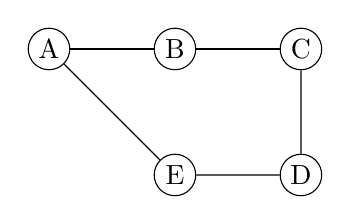
\begin{tikzpicture}[scale=0.8]
      \node[latent, minimum size=15pt] (A) at (0,0) {A};
      \node[latent, minimum size=15pt] (B) at (2,0) {B};
      \node[latent, minimum size=15pt] (C) at (4,0) {C};
      \node[latent, minimum size=15pt] (E) at (2,-2) {E};
      \node[latent, minimum size=15pt] (D) at (4,-2) {D};
      \edge[-]{A}{B,E}
      \edge[-]{C}{B,D}
      \edge[-]{E}{D}
    \end{tikzpicture}
  \end{center}
\end{solution}


\item \textbf{[3 pts]} Triangulate $ \Hcal $ to construct a chordal graph $ \Hcal^* $. 

(Although there are many ways to triangulate a graph, for the ease of grading, please use the triangulation that corresponds to the elimination order $ A, B, C, D, E $.)
\begin{solution}
  Here is the \textbf{triangulated graph} $\Hcal^{*}$:\\
  \begin{center}
    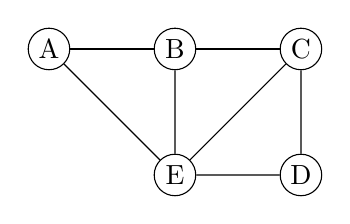
\begin{tikzpicture}[scale=0.8]
      \node[latent, minimum size=15pt] (A) at (0,0) {A};
      \node[latent, minimum size=15pt] (B) at (2,0) {B};
      \node[latent, minimum size=15pt] (C) at (4,0) {C};
      \node[latent, minimum size=15pt] (E) at (2,-2) {E};
      \node[latent, minimum size=15pt] (D) at (4,-2) {D};
      \edge[-]{A}{B,E}
      \edge[-]{C}{B,D,E}
      \edge[-]{E}{D,B}
    \end{tikzpicture}
  \end{center}
\end{solution}



\item \textbf{[3 pts]} Construct a cluster graph $ \Ucal $ where each node is a maximal clique $ \Cbs_i $ from $ \Hcal^* $ and each edge is the sepset $ \Sbs_{i,j} = \Cbs_i \cap \Cbs_j $ between adjacent cliques $ \Cbs_i $ and $ \Cbs_j $. 
\begin{solution}
  here is the \textbf{cliqure tree} obtained from the \emph{chordal} graph
  $\Hcal^{*}$.\\[4pt]

  \begin{center}
  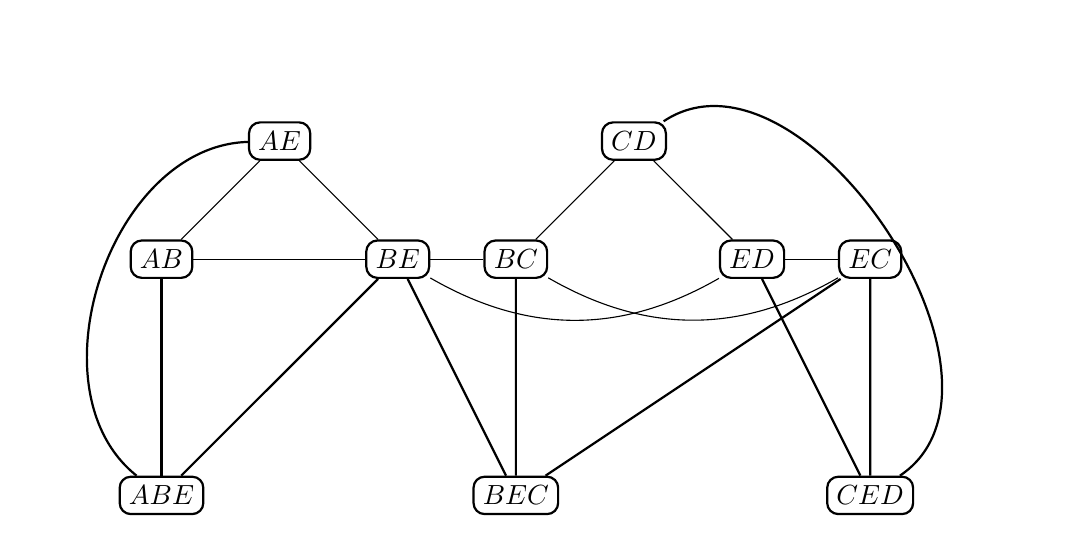
\begin{tikzpicture}[scale=1.5]
    %binary cliques
    \node[rounded corners, draw, thick] (AB) at (0,0) {$AB$};
    \node[rounded corners, draw, thick] (AE)at (1,1) {$AE$};
    \node[rounded corners, draw, thick] (BE)at (2,0) {$BE$};
    \node[rounded corners, draw, thick] (BC)at (3,0) {$BC$};
    \node[rounded corners, draw, thick] (CD)at (4,1) {$CD$};
    \node[rounded corners, draw, thick] (ED)at (5,0) {$ED$};

    \node[rounded corners, draw, thick] (EC)at (6,0) {$EC$};

    \path[draw](AB)--(AE);
    \path[draw](EC)--(ED);
    \path[draw](EC)edge[bend left](BC);
    \path[draw](AE)--(BE);
    \path[draw](AB)--(BE);
    \path[draw](BE)--(BC);
    \path[draw](BC)--(CD);
    \path[draw](CD)--(ED);
    \path[draw](BE)edge[bend right](ED);


    %thre cliques
    \node[rounded corners, draw, thick] (ABE) at (0, -2){$ABE$};
    \node[rounded corners, draw, thick] (BEC) at (3, -2){$BEC$};
    \node[rounded corners, draw, thick] (CED) at (6, -2){$CED$};
    \path[draw,thick] (AB)--(ABE);
    \path[draw,thick] (AE)edge[bend right=70](ABE);
    \path[draw,thick] (BE)--(ABE);
    \path[draw,thick] (BC)--(BEC);
    \path[draw,thick] (BE)--(BEC);
    \path[draw,thick] (EC)--(BEC);
    \path[draw,thick] (EC)--(CED);
    \path[draw,thick] (ED)--(CED);
    \path[draw,thick] (CD)edge[bend left=90](CED);
  \end{tikzpicture}
  \end{center}
  
\end{solution}



\item \textbf{[3 pts]} Run maximum spanning tree algorithm on $ \Ucal $ to construct a junction tree $ \Tcal $. 

(The cluster graph is small enough to calculate maximum spanning tree in one's head.)

\begin{solution}
  Here is the maximum junction tree:\\[4pt]

\begin{center}
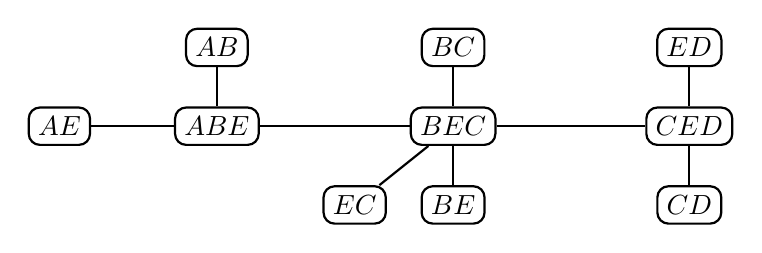
\begin{tikzpicture}[scale=1, transform shape]
  \foreach \x/\y/\z in {0/0/ABE, 3/0/BEC, 6/0/CED}
  {
    \node[rounded corners, draw, thick] (\z) at(\x, \y) {$\z$};
  }
  \path[draw,thick](ABE)--(BEC);
  \path[draw,thick](BEC)--(CED);
  \node[rounded corners, thick,draw] (AE) at (-2,0) {$AE$};
  \node[rounded corners, thick,draw] (AB) at (0,1) {$AB$};
  \node[rounded corners, thick,draw] (BE) at (3,-1) {$BE$};
  \node[rounded corners, thick,draw] (BC) at (3,1) {$BC$};
  \node[rounded corners, thick,draw] (CD) at (6,-1) {$CD$};
  \node[rounded corners, thick,draw] (ED) at (6,1) {$ED$};
  \node[rounded corners, thick,draw] (EC) at (1.75,-1) {$EC$};
  \path[thick,draw] (AE)--(ABE);
  \path[thick,draw] (AB)--(ABE);
  \path[thick,draw] (BE)--(BEC);
  \path[thick,draw] (BC)--(BEC);
  \path[thick,draw] (CD)--(CED);
  \path[thick,draw] (EC)--(BEC);
  \path[thick,draw] (ED)--(CED);
\end{tikzpicture}
\end{center}
\end{solution}
\end{enumerate}



\subsection{Junction tree in action: part 2 [20 points]}

Continuing from part 1, now assume all variables are binary and the CPDs are parameterized as follows:
\begin{table}[h]
\centering
\hspace{-2em}
\begin{subtable}[]{0.14\textwidth}
\begin{tabular}{@{}ccc@{}}
\toprule
$A$ & $P(A)$ \\ \midrule
0  &  $ x_0 $     \\ \bottomrule
\end{tabular}
\end{subtable}
~
\begin{subtable}[]{0.2\textwidth}
\begin{tabular}{@{}ccc@{}}
\toprule
$A$ & $B$ & $P(B|A)$ \\ \midrule
0   & 0   &   $ x_1 $      \\
1   & 0   &   $ x_2 $     \\ \bottomrule
\end{tabular}
\end{subtable}
~
\begin{subtable}[]{0.2\textwidth}
\begin{tabular}{@{}ccc@{}}
\toprule
$A$ & $E$ & $P(E|A)$ \\ \midrule
0   & 0   & $ x_3 $      \\
1   & 0   & $ x_4 $      \\ \bottomrule
\end{tabular}
\end{subtable}
~
\begin{subtable}[]{0.2\textwidth}
\begin{tabular}{@{}ccc@{}}
\toprule
$B$ & $C$ & $P(C|B)$ \\ \midrule
0   & 0   &  $ x_5 $      \\
1   & 0   &  $ x_6 $      \\ \bottomrule
\end{tabular}
\end{subtable}
~
\begin{subtable}[]{0.2\textwidth}
\begin{tabular}{@{}cccc@{}}
\toprule
$C$ & $E$ & $ D $ & $P(D|C, E)$ \\ \midrule
0   & 0   &  0 &  $ x_7 $      \\
0   & 1   &  0 &  $ x_8 $     \\ 
1   & 0   &  0 &  $ x_9 $      \\
1   & 1   &  0 &  $ x_{10} $      \\ \bottomrule
\end{tabular}
\end{subtable}
\end{table}

We are going to implement belief propagation on $ \Tcal $.
The provided template \verb|junction_tree.py| contains the following tasks:


\begin{itemize}
\item \verb|initial_clique_potentials()|: Compute  initial clique potentials $ \psi_i (\Cbs_i) $ from factors $ \phi_i  $. 

\item \verb|messages()|: Compute messages $ \delta_{i \to j}  $ from initial clique potentials $ \psi_i (\Cbs_i)  $.

\item \verb|beliefs()|: Compute calibrated clique beliefs $ \beta_i(\Cbs_i) $ and sepset beliefs $ \mu_{i,j} (\Sbs_{i,j})  $, using initial clique potentials $ \psi_i (\Cbs_i) $ and messages $ \delta_{i \to j}  $. 

\item Using the beliefs $ \beta_i(\Cbs_i), \mu_{i,j} (\Sbs_{i,j}) $, compute 
\begin{itemize}
\item \verb|query1()|: $ P(B) $
\item \verb|query2()|: $ P(A | C) $
\item \verb|query3()|: $ P(A, B, C, D, E) $
\end{itemize}

\end{itemize}

Please finish the unimplemented TODO blocks and submit completed \verb|junction_tree.py| to Gradescope (\verb|https://www.gradescope.com/courses/36025|). 


In the implementation, please represent factors as \verb|numpy.ndarray| and store different factors in a dictionary with its scope as the key.
For example, as provided in the template, \verb|phi['ab']| is a factor $ \phi_{AB} $ represented as a $ 2 \times 2 $ matrix, where \verb|phi['ab'][0, 0]| $ = \phi_{AB} (A = 0, B = 0) =  P(B= 0 | A = 0)  = x_1 $.
For messages, one can use \verb|delta['ab_cd']| to denote a message from $ AB $ to $ CD $.
Most functions can be written in 3 lines of code. 
You may find \verb|np.einsum()| useful.

\newpage

\section{Parameter Learning [15 points] (Xun)}


\begin{figure}[h]
\centering
\begin{tikzcd}
Y_1 \arrow[r] \arrow[d] & Y_2 \arrow[r] \arrow[d] & \cdots \arrow[r] & Y_T \arrow[d] \\
X_1  &  X_2  & & X_T
\end{tikzcd}
\end{figure}

Consider an HMM with $ Y_t \in [M] $, $ X_t \in \mathbb{R}^{K} $ ($ M, K \in \mathbb{N} $).
Let $ (\pi, A, \{\mu_i, \sigma_i^2\}_{i=1}^M) $ be its parameters, where $ \pi \in \mathbb{R}^{M} $ is the initial state distribution, $ A \in \mathbb{R}^{M \times M} $ is the transition matrix, $ \mu_i \in \mathbb{R}^{K} $ and $ \sigma_i^2 > 0 $ are parameters of the emission distribution, which is defined to be an isotropic Gaussian. 
In other words,
\begin{align}
P(Y_1 = i) & = \pi_{i} \\
P(Y_{t+1} = j | Y_t = i) & = A_{ij} \\
P(X_t | Y_t = i) & = \Ncal(X_t; \mu_i, \sigma_i^2 I).
\end{align}


We are going to implement the Baum-Welch (EM) algorithm that estimates parameters from data $ \boldsymbol{X} \in \mathbb{R}^{N \times T \times K} $, which is a collection of $ N $ observed sequences of length $ T $. 
Note that there are different forms of forward-backward algorithms, for instance the $ (\alpha,\gamma) $-recursion, which is slightly different from the $ (\alpha,\beta)$-recursion we saw in the class. 
For the ease of grading, however, please implement the $ (\alpha,\beta) $ version, and remember to normalize the messages at each step for numerical stability.


Please complete the unimplemented TODO blocks in the template \verb|baum_welch.py| and submit it to Gradescope (\verb|https://www.gradescope.com/courses/36025|).
The template has its own toy problem to verify the implementation. 
The test cases are ran on other randomly generated problem instances.



\newpage
\bibliography{pgm}
\bibliographystyle{abbrvnat}


\end{document}
